%!TEX encoding = UTF-8 Unicode
%==================================================
%      PREAMBOLO e DICHIARAZIONI INIZIALI
%==================================================
\documentclass[10pt,oneside,a4paper]{article}

\usepackage[utf8]{inputenc} 
\usepackage[italian]{babel}
\usepackage[T1]{fontenc}
\usepackage{siunitx} %Inserisce automaticamente i dati con le unità  di misura correttamente formattate del SI (utilizzo: \SI{0.82}{m^2}, in generale \SI{misura con il punto decimale}{unità  di misura})
\sisetup{output-decimal-marker = {.}, separate-uncertainty = true, input-uncertainty-signs = \pm, detect-weight=true, detect-family=true} %per usare SI con il punto decimale
\usepackage{listings} %Per citare codice informatico formattandolo correttamente
\usepackage{amsmath,amsthm,verbatim,amssymb,amsfonts,amscd,graphicx,mathtools}
\usepackage[makeroom]{cancel}
\newcommand{\abs}[1]{\left\lvert\,#1\,\right\rvert}
\usepackage{geometry}
\usepackage{epigraph}
\usepackage{booktabs}	%tabelle migliorate
\usepackage{tablefootnote}	%note a piè di pagina in tabella
\usepackage{threeparttable} %tabella con note a piè di tabella
\usepackage{caption}	%descrizione per figure
\usepackage{dblfnote}
\captionsetup{tableposition=top,figureposition=bottom,font=small} %setup descrizione
\usepackage{float}
\usepackage{esvect} %vettori
\usepackage{longtable} %tabelle lunghe
\usepackage[dvipsnames]{xcolor}
\definecolor{sepia}{HTML}{80002A}
\usepackage[colorlinks=true, citecolor=black, linkcolor=sepia, urlcolor=black]{hyperref}
\usepackage{mathrsfs}
\usepackage{circuitikz}
\tikzset{
  font={\fontsize{7pt}{12}\selectfont}}
\ctikzset{bipoles/resistor/height=0.2}
\ctikzset{bipoles/resistor/width=0.4}
\ctikzset{bipoles/diode/height=0.3}
\ctikzset{bipoles/diode/width=0.3}
\ctikzset{tripoles/american nand port/height=0.7}
\ctikzset{tripoles/american nand port/width=0.8}
\usepackage{enumitem} %Liste senza spazi verticali
\setlist{noitemsep}
\usepackage{amsmath}


\interfootnotelinepenalty=10000


\usepackage{multicol}
\newenvironment{Figure}
  {\par\medskip\noindent\minipage{\linewidth}}
  {\endminipage\par\medskip}

\newcommand{\var}{\operatorname{var}}
\newcommand{\cov}{\operatorname{cov}}


\usepackage{listings} %Per inserire codice
\lstdefinestyle{CStyle}{
    backgroundcolor=\color{backgroundColour},   
    commentstyle=\color{mGreen},
    keywordstyle=\color{magenta},
    numberstyle=\tiny\color{mGray},
    stringstyle=\color{mPurple},
    basicstyle=\footnotesize\ttfamily,
    breakatwhitespace=false,         
    breaklines=true,                 
    captionpos=b,                    
    keepspaces=true,                 
    numbers=left,                    
    numbersep=5pt,                  
    showspaces=false,                
    showstringspaces=false,
    showtabs=false,                  
    tabsize=2,
    language=C
}

\definecolor{color1}{RGB}{90,0,0} % Color of the article title and sections
\definecolor{color2}{RGB}{0,20,50} % Color of the boxes behind the abstract and headings
\definecolor{mGreen}{rgb}{0,0.6,0}
\definecolor{mGray}{rgb}{0.5,0.5,0.5}
\definecolor{mPurple}{rgb}{0.58,0,0.82}
\definecolor{backgroundColour}{rgb}{0.95,0.95,0.92}


%==================================================
%                  PRIMA PAGINA
%==================================================

\title{\textsc{\textbf{Esercitazione 8}: Familiarizzazione con Arduino}}
\author{\small{G. Galbato Muscio} \and \small{L. Gravina} \and \small{L. Graziotto}}
\date{11 Dicembre 2018}

\begin{document}
	\begin{figure}
		\centering
		
\includegraphics[scale=0.5, trim={2.8cm 8.9cm 0 9cm}, clip]{logo.png}
	\end{figure}
	\maketitle
	\begin{center} 
		\fbox{{\fontsize{12pt}{8mm}\textsc{Gruppo 11}}} \\
	\end{center}
\hrule
\vspace{0.5cm}
\renewcommand{\abstractname}{Abstract}
\begin{abstract}
Si studia il tempo impiegato dal microcontrollore Arduino UNO a svolgere determinate istruzioni, da operazioni aritmetiche, a calcolo di funzioni, a operazioni di Input/Output. Si studia il comportamento dei pin dotati di \emph{pulse width modulation}. Si realizza, mediante la funzione di lettura analogica, un ADC, e se ne calcolano i valori di calibrazione. Si compie infine un campionamento digitale di un segnale analogico periodico.
\end{abstract}
\vspace{4cm}
\tableofcontents %Indice
\newpage


\pagebreak


\begin{multicols}{2}
%==================================================
%             COMUNICAZIONE SERIALE
%==================================================
\section{Comunicazione seriale}
Si realizza un programma per Arduino (Listato~\ref{lst:esecuzione}) finalizzato a misurare i tempi impiegati per lo svolgimento di alcune istruzioni, e la dipendenza di tali tempi dall'ordine di grandezza dei numeri da manipolare. La funzione \texttt{micros()} permette di registrare i tempi di esecuzione, che vengono riportati in Tabella~\ref{tab:comunicazione}: in questa prima fase, i numeri sono di tipo \texttt{float} con una cifra dopo la virgola, e il tempo di esecuzione è misurato escludendo quello impiegato per la scrittura su schermo del risultato. 

\begin{lstlisting}[style=CStyle, caption={Codice per la misura dei tempi di esecuzione di operazioni elementari}, label=lst:esecuzione]
float a, b, c;
long unsigned t0, t1;
void setup() {
	Serial.begin(9600);
	a = 2.68;
	b = 11.9;
}

void loop() {
	t0 = micros();
		c = a+b; //somma
		//c = a*b; //prodotto
		//c = a/b; //divisione
		//c = sqrt(a); //radice quadra
		//c = sin(a); //seno
		//c = max(a,b); //massimo
		//c = a*a; //quadrato
		//c = pow(a,2); //quadrato con funzione pow
	t1 = micros();
	Serial.print(t0);
	Serial.print(" ");
	Serial.print(t1);
	Serial.print(" ");
	Serial.println(t1-t0);
}

\end{lstlisting}

\begin{center}
\captionof{table}{Misure per la stima dei tempi di esecuzione}
\label{tab:comunicazione}
\begin{tabular}{c|c|c|c}
Operazione & $t_0$ [\SI{}{\micro s}] &  $t_1$ [\SI{}{\micro s}] &  $\Delta t$ [\SI{}{\micro s}] \\
\hline
$a + b$ & 312 & 324 & 12 \\
$a \cdot b$ & 312 & 328 & 16 \\
$a / b$ & 336 & 372 & 36\\
$\sqrt{a}$ & 796 & 834 & 38\\
$sin(a)$ & 500 & 612 & 112\\
$max\{a,b\}$ & 264 & 272 & 8 \\
$a^2$ & 1208 & 1220 & 12 \\
$pow(a,2)$ & 1208 & 1220 & 12 \\
\hline
\end{tabular}
\end{center}

Per ottenere una stima più precisa, si ripete ogni operazione inserendola all'interno di un ciclo $\texttt{for}$ che la iteri per $N=1000$ volte; quindi si ottiene il tempo medio di esecuzione come $(t_1 - t_0)/N$. Si riportano i risultati in Tabella~\ref{tab:com1000}; anche in questo caso non sono inclusi i tempi necessari alla scrittura a schermo. Si osserva che in questo secondo caso i tempi sono maggiori fino al $25\%$ (nel caso della somma), poiché è incluso il tempo di esecuzione del ciclo $\texttt{for}$.

\begin{center}
\captionof{table}{Misure per la stima dei tempi di esecuzione, con $N=1000$ iterazioni}
\label{tab:com1000}
\begin{tabular}{c|c|c|c}
Operazione & $t_0$ [\SI{}{\micro s}] &  $t_1$ [\SI{}{\micro s}] &  $\Delta t / N$ [\SI{}{\micro s}] \\
\hline
$a + b$ & 17148 & 32956 & 15.8 \\
$a \cdot b$ & 18908 & 34692 & 17.6 \\
$a / b$ & 80832 & 119840 & 39.0 \\
$\sqrt{a}$ & 158988 & 197184 & 38.2 \\
$sin(a)$ & 235864 & 352236 & 116.4 \\
$max\{a,b\}$ & 63096 & 71048 & 8.0 \\
$a^2$ & 18088 & 34852 & 16.8\\
$pow(a,2)$ & 18088 & 34852 & 16.8\\
\hline
\end{tabular}
\end{center}

Per l'operazione di moltiplicazione, si studia la dipendenza del tempo di esecuzione dal numero di cifre: con il ciclo \texttt{for} si varia il numero $a$, in questo caso intero, da moltiplicare per $10$, da $0$ a $10^5$ a passi di $1$, e si misura volta per volta il tempo di esecuzione (si veda il Listato~\ref{lst:moltiplicazione}). Si osserva in questo caso che il tempo rimane circa costante.

\begin{lstlisting}[style=CStyle, caption={Codice per la misura dei tempi di esecuzione della moltiplicazione}, label=lst:moltiplicazione]
#define MAX 10000

int p, q;
long unsigned t0, t1;

void setup() {
	Serial.begin(9600);
	p=10; 
}

void loop() { 
	Serial.print(p);
	t0 = micros();
	q = p*10;
	t1 = micros();
	p = p+1;	
	Serial.print(p);
	Serial.print(" ");
	Serial.println(t1-t0); //stampa il tempo
	while (p > MAX) { }; //il programma si arresta quando il numero supera MAX
	}
\end{lstlisting}

%\begin{Figure}
%	\begin{center}
%	\includegraphics[width=\linewidth]{}
%	\captionof{figure}{Tempo di esecuzione per la moltiplicazione in funzione del numero $a$}
%	\label{fig:moltiplicazione}
%	\end{center}
%\end{Figure}

Per stimare il tempo impiegato a scrivere su schermo si realizza una stringa di caratteri di lunghezza via via maggiore, che viene quindi stampata a video, come da Listato~\ref{lst:caratteri}. Si riporta in Figura~\ref{fig:scrittura} il grafico del tempo di esecuzione dell'istruzione di output a video in funzione del numero di caratteri della stringa.

\begin{lstlisting}[style=CStyle, caption={Codice per la misura dei tempi di scrittura a video}, label=lst:caratteri]
#define LMAX 100 //Lunghezza stringa

int i=0;
long unsigned t0, t1;
String string;

void setup() {
  Serial.begin(9600);
}

void loop() {
    string += "a";
    t0 = micros();
    Serial.print(string);
    t1 = micros();
    
    i = i+1;
    Serial.print(" ");
    Serial.print(i);
    Serial.print(" ");
    Serial.println(t1-t0);
    
    while(i>LMAX) { }
}
\end{lstlisting}

\begin{Figure}
	\begin{center}
	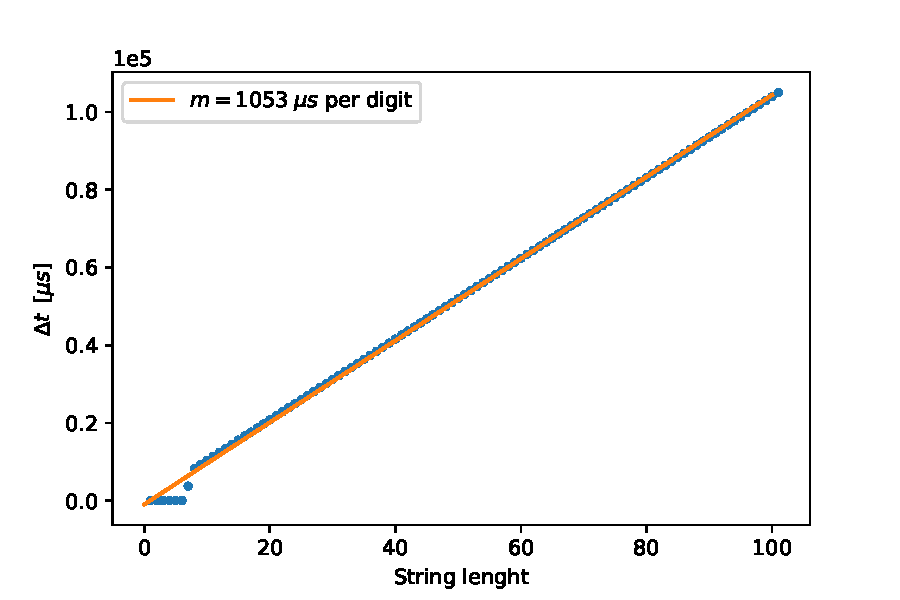
\includegraphics[width=\linewidth]{stringa.pdf}
	\captionof{figure}{Tempo di esecuzione per la scrittura a video in funzione del numero di caratteri, la scala sull'asse $y$ si intende moltiplicata per $10^5$}
	\label{fig:scrittura}
	\end{center}
\end{Figure}

Interpolando linearmente si ottiene un coefficiente angolare pari a $m = \SI{1053}{\micro\s}$, che ha il significato di tempo necessario per trasmettere un singolo carattere: considerando una velocità di trasmissione pari a \SI{9600}{baud}, tale tempo è coerente con l'aspettativa teorica pari a $t^\text{teo} = \frac{8}{9600} = \SI{833}{\micro\s}$, ottenuto considerando che un char è composto da $8$ bit e che, a questa velocità, viene trasmesso un bit ogni $1/9600$ secondi.

%==================================================
%              ANALOG WRITE
%==================================================
\section{Operazioni di Input Analogico}
Si utilizzano i pin digitali in modalità \emph{pulse width modulation} (PWM), che permette di ottenere un'onda quadra con \emph{duty cycle} variabile scegliendo un valore compreso tra $0$ e $255$, si veda il Listato~\ref{lst:PWM}. La frequenza è fissata: per il pin \texttt{9} è di \SI{490 \pm 14}{Hz}, mentre per il pin \texttt{6} di \SI{976 \pm 30}{Hz}, misurate entrambe con l'oscilloscopio. 

Si connette innanzitutto al pin dotato di PWM un LED protetto verso massa da una resistenza $R = \SI{0.998 \pm 0.005}{\kilo\ohm}$, misurata con il multimetro: si osserva l'aumento di luminosità del LED al crescere del \emph{duty cycle}, poiché il tempo per periodo in cui il livello logico è alto aumenta\footnote{La frequenza è sufficientemente alta da non distinguere tra livello logico alto e basso, ossia non si percepisce la luminosità del LED come oscillante.}. Successivamente si connette direttamente il pin \texttt{9} al canale \texttt{CH1} dell'oscilloscopio, e si riportano le istantanee per valori del \emph{duty cycle} del $20\%$ e del $78\%$ rispettivamente nelle Figure~\ref{fig:quadra1} e~\ref{fig:quadra2}. 

\begin{lstlisting}[style=CStyle, caption={Codice per la scrittura PWM}, label=lst:PWM]
int ledPin = 9;
int val = 128;
void setup() {
  pinMode(ledPin, OUTPUT);
  Serial.begin(9600);
  Serial.println("Ready");
  Serial.println(" ");
}

void loop() {
  if (Serial.available() > 0) {
    val=Serial.parseInt();
  // check value in
     if (val>=0 && val <=255) {
      analogWrite(ledPin, val);
      Serial.print("Scritto valore :");
      Serial.println(val);
     }
     else {
      Serial.println("Valore fuori range (0:255)!!!");
     }
  }
}
\end{lstlisting}

\begin{Figure}
	\begin{center}
	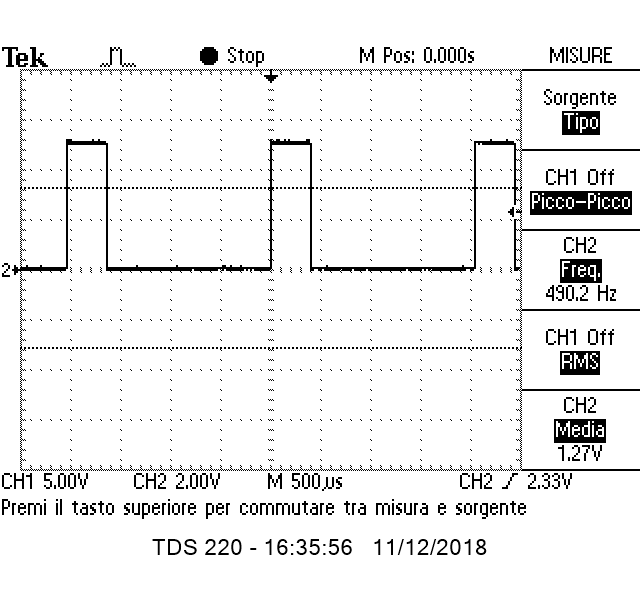
\includegraphics[width=0.9\linewidth]{quadra1.png}
	\captionof{figure}{Istantanea dell'oscilloscopio per il pin \texttt{9} in PWM: \emph{duty cycle} del $20\%$}
	\label{fig:quadra1}
	\end{center}
\end{Figure}

\begin{Figure}
	\begin{center}
	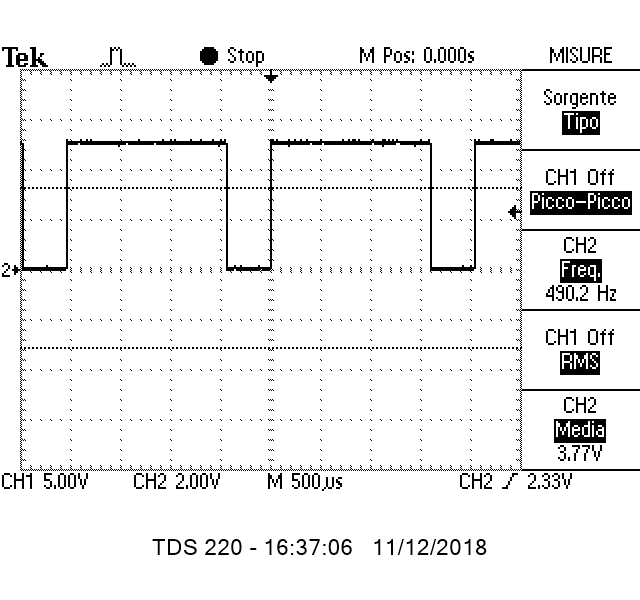
\includegraphics[width=0.9\linewidth]{quadra2.png}
	\captionof{figure}{Istantanea dell'oscilloscopio per il pin \texttt{9} in PWM: \emph{duty cycle} del $78\%$}
	\label{fig:quadra2}
	\end{center}
\end{Figure}

Si ripete l'operazione di scrittura analogica con la PWM utilizzando un'onda triangolare per modulare la durata del \emph{duty cycle}, come da Listato~\ref{lst:triangolare}; per ottenere un'onda triangolare visibile sull'oscilloscopio a partire da quella triangolare di modulazione PWM, si realizza un filtro RC integratore. Si sceglie
\begin{itemize}
\item[--] $R = \SI{0.328 \pm 0.002}{\kilo\ohm}$;
\item[--] $C = \SI{83.7 \pm 0.4}{\micro\farad}$,
\end{itemize}
misurati con multimetro e ponte, in modo da avere una bassa frequenza di taglio, molto inferiore alla frequenza dell'onda modulata (che è di \SI{200}{Hz}\footnote{Nel codice il periodo dell'onda è rappresentato dalla variabile \emph{millisecondi}.}):
\[
f_T = \frac{1}{RC} = \SI{36.4 \pm 0.4}{\Hz}.
\] 
Si riporta in Figura~\ref{fig:PWM_filtro_triangolare} lo screenshot dell'oscilloscopio per il segnale in uscita.

\begin{lstlisting}[style=CStyle, caption={Codice per la scrittura PWM, modulazione triangolare}, label=lst:triangolare]
int ledPin = 9;
int val,i;
int millisecondi = 5;

void setup() {
  i = val = 0;
  pinMode(ledPin, OUTPUT);
  Serial.begin(9600);
  Serial.println("Ready");
}

void loop() {
  for(i=0;i<255;i++){
    val = i;
    analogWrite(ledPin,val);
    delay(millisecondi);    
  }
    for(i=0;i<255;i++){
    val = 255-i;
    analogWrite(ledPin,val);
    delay(millisecondi); 
  }
}
\end{lstlisting}

\begin{Figure}
	\begin{center}
	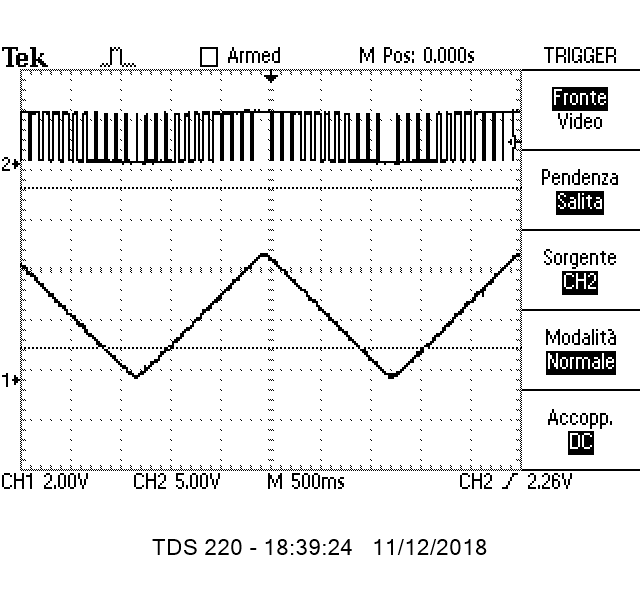
\includegraphics[width=0.9\linewidth]{triangolare2.png}
	\captionof{figure}{Istantanea dell'oscilloscopio per il pin \texttt{9} in PWM, onda triangolare}
	\label{fig:PWM_filtro_triangolare}
	\end{center}
\end{Figure}

Si ripete la stessa identica procedura per un segnale modulato con una PWM sinusoidale. Il programma è riportato nel Listato~\ref{lst:sinusoidale}, e l'istantanea dell'oscilloscopio per questa configurazione in Figura~\ref{fig:PWM_filtro_sinusoidale}.

\begin{lstlisting}[style=CStyle, caption={Codice per la scrittura PWM, modulazione sinusoidale}, label=lst:sinusoidale]
int ledPin = 9;
int val;
float x;
float dx = 0.01;
int millisecondi = 1;

void setup() {
  val = 0;
  x=0.;
  pinMode(ledPin, OUTPUT);
  Serial.begin(9600);
  Serial.println("Ready");
}

void loop() {
  val = (int)(127.5*sin(x)+127.5);
  Serial.println(val);
  analogWrite(ledPin,(int)(val));
  x += dx;
  delay(millisecondi);
}
\end{lstlisting}

\begin{Figure}
	\begin{center}
	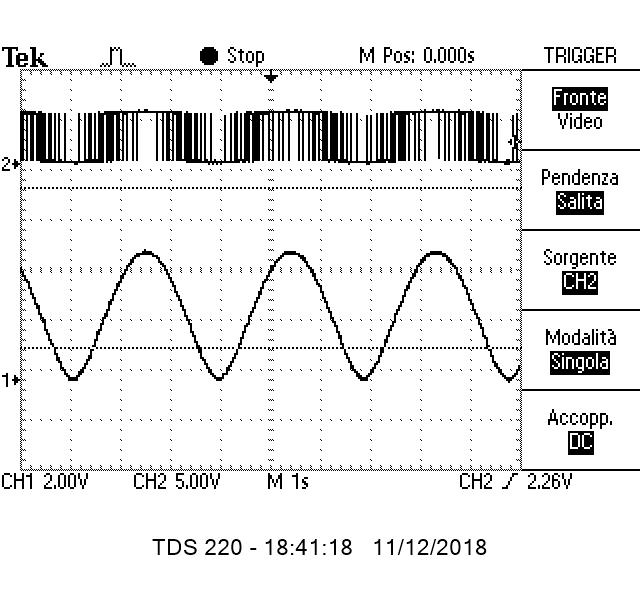
\includegraphics[width=0.9\linewidth]{sinusoide2.png}
	\captionof{figure}{Istantanea dell'oscilloscopio per il pin \texttt{9} in PWM, onda sinusoidale}
	\label{fig:PWM_filtro_sinusoidale}
	\end{center}
\end{Figure}

In entrambi gli screenshot è riportata in alto l'uscita del pin \texttt{9} di Arduino, che rappresenta l'onda quadra \emph{pulse width modulated}: si notano gli addensamenti e le rarefazioni di linee in corrispondenza dei massimi e dei minimi delle funzioni triangolare e sinusoidale.


%==================================================
%             CALIBRAZIONE ADC
%==================================================
\section{Calibrazione ADC}
Si utilizza il pin \texttt{A3} di ingresso analogico, al quale è inviata una tensione continua compresa tra $0$ e $5 \SI{}{V}$ mediante il generatore di tensione. Mediante il Listato~\ref{lst:calibrazioneADC}, si converte il valore analogico della tensione $V_\text{in}$ in un valore digitale $\text{Val}_V$ a $10$ bit (dunque compreso tra $0$ e $2^{10}-1 = 1023$), proporzionale al primo. La tensione in ingresso $V_\text{in}$ è misurata con il multimetro; nel caso ideale la tensione corrispondente al valore digitale acquisito da Arduino dovrebbe essere
\[
V_x = \frac{\text{Val}_V}{1023} \cdot V_\text{ref},
\]
dove $V_\text{ref} = \SI{5.0}{V}$ è la tensione di riferimento qui impostata. Si confronterà successivamente l'aderenza dei dati sperimentali a questa formula.
Si riportano in Tabella~\ref{tab:calibrazioneADC} le misure per la calibrazione dell'ADC. Il programma scritto è riportato nel Listato~\ref{lst:calibrazioneADC}. 

\begin{lstlisting}[style=CStyle, caption={Codice per la conversione analogico-digitale}, label=lst:calibrazioneADC]
int analogPin = 3;
int RdVal = 0;
float Vx = 0.0;
void setup() {
  analogReference(DEFAULT); // 5 V
  Serial.begin(9600);
  Serial.println("Arduino Voltage meter");
  Serial.println(" ");
}

void loop() {
  RdVal = analogRead(analogPin);
  Vx = float(5.0)*(float(RdVal)/float(1023));
  delay(2000);
  // Serial.print(RdVal);
  Serial.print(" Tensione letta: ");
  Serial.println(Vx);
}
\end{lstlisting}

\begin{center}
\captionof{table}{Misure per la calibrazione dell'ADC}
\label{tab:calibrazioneADC}
\begin{tabular}{c|c|c}
$V_\text{in}$ [\SI{}{V}] & $\text{Val}_V$ &  $V_x$ [\SI{}{V}] \\
$(\pm 0.5\%)$&&\\
\hline
5.00 & 1022 & 5.00 \\
4.50 & 921 & 4.50 \\
4.00 & 818 & 4.00 \\
3.50 & 716 & 3.50 \\
3.01 & 615 & 3.00 \\
2.50 & 511 & 2.50 \\
2.00 & 408 & 1.99 \\
1.50 & 306 & 1.50 \\ 
1.00 & 203 & 0.99 \\
0.500 & 100 & 0.49 \\
0.0410 & 6 & 0.03 \\
\hline
\end{tabular}
\end{center}

Nel grafico di Figura~\ref{fig:calibrazioneADC} sono riportati i punti sperimentali e la retta $y = mx+q$ che meglio li interpola, di coefficiente angolare $m = \SI{205.0 \pm 0.1}{V^{-1}}$ e intercetta $q = \SI{-2.0 \pm 0.3}{}$; li si confronta con i valori previsti $m^{\text{(atteso)}} = 1023/\SI{5.0}{V} = \SI{204.6}{V^{-1}}$ e $q^{\text{(atteso)}} = 0$. Il chi quadro è, inoltre, $\chi^2 = 2.4$, che si confronta con il numero di gradi di libertà ($9$), da cui si ipotizza che le incertezze sul valore di $\text{Val}_V$, supposte di 1 bit, siano sottostimate.

\begin{Figure}
	\begin{center}
	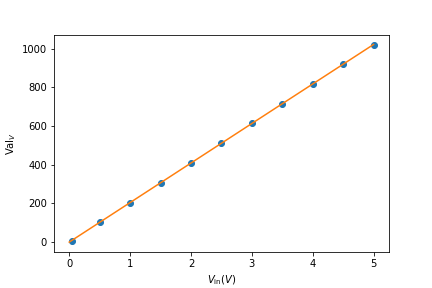
\includegraphics[width=\linewidth]{calibrazioneADC.png}
	\captionof{figure}{$\text{Val}_V$ in funzione di $V_\text{in}$}
	\label{fig:calibrazioneADC}
	\end{center}
\end{Figure}

Invertendo la relazione per il coefficiente angolare, si ottiene la costante di calibrazione $k$ dell'ADC, per cui si avrà, nel seguito
\[
V_x = \text{Val}_V \cdot k = \text{Val}_V \cdot \SI{4.878 \pm 0.002 e-3}{V}.
\]

%==================================================
%             ACQUISIZIONE ADC
%==================================================
\section{Acquisizione dati dall'ADC}
Si esegue un campionamento digitale di un segnale analogico, utilizzando l'ADC studiato nella sezione precedente. La frequenza del campionamento è variabile fino ad un massimo imposto dalle caratteristiche di Arduino di circa \SI{9}{\kilo \Hz}, dunque si sceglierà una frequenza inferiore, come da listato seguente.

Si invia pertanto, mediante il generatore di segnali, un segnale sinusoidale di ampiezza picco-picco \SI{4.24 \pm 0.01}{V} e frequenza \SI{69 \pm 2}{\Hz}; si agisce inoltre sull'offset affinché l'onda abbia tensione sempre positiva. Il codice scritto per Arduino, riportato nel Listato~\ref{lst:acquisizioneADC}, esegue il campionamento salvando i punti in un buffer, che viene scritto su schermo solo in un secondo momento\footnote{Questo è fatto per non far incidere il tempo di trasmissione seriale sulla velocità di campionamento. In ogni caso, si ha cura di non acquisire troppi punti data la memoria limitata di Arduino. Per campionamenti più numerosi, si potrebbe usare una scrittura volta per volta aumentando la velocità di trasmissione oltre i \SI{9600}{Baud}.}; quindi esso viene analizzato. Si riporta in Figura~\ref{fig:ADC_sinusoidale} l'acquisizione del segnale sinusoidale, con $V_x$ calcolata a partire dal valore digitale mediante la costante di calibrazione ricavata in precedenza, sovrapposta al segnale misurato dall'oscilloscopio\footnote{Avendo cura di traslare l'asse dei tempi e di far concordare le unità di misura}. Si riporta inoltre in Figura~\ref{fig:oscilloscopio_ADC_sinusoidale} un'istantanea dell'oscilloscopio per questa configurazione.

\begin{lstlisting}[style=CStyle, caption={Codice per l'acquisizione dall'ADC}, label=lst:acquisizioneADC]
#define CALIBRATION 0.004878 //Valore di calibrazione per l'ADC
#define OFFSET 105 //Tempo in millisecondi per le operazioni di lettura contenute nel ciclo for del loop

int data[100];
int analogPin = 3;
int NSamples = 100;
float f = 80;
int T = int (1000000./(float)(f*NSamples))-OFFSET;
int i = 0;
long unsigned t0,t1;

void setup() {
Serial.begin(9600);
}

void loop() {
  t0 = micros();
  for (i=0;i<NSamples;i++){
    data[i] = analogRead(analogPin);
    delayMicroseconds(T);
  }
  t1 = micros();
  for(i=0;i<NSamples;i++){
    Serial.print(i);
    Serial.print(" ");
    Serial.print(t);
    Serial.print(" ");
    Serial.print(data[i]);
    Serial.print(" ");
    //Serial.print(" V = ");
    float temp = float (data[i])*CALIBRATION;
    Serial.print(temp);
    Serial.print(" ");
    Serial.print(float(t1-t0)/NSamples);
  }
  delay(1000);
  while(1){ }
}
\end{lstlisting}

\begin{Figure}
	\begin{center}
	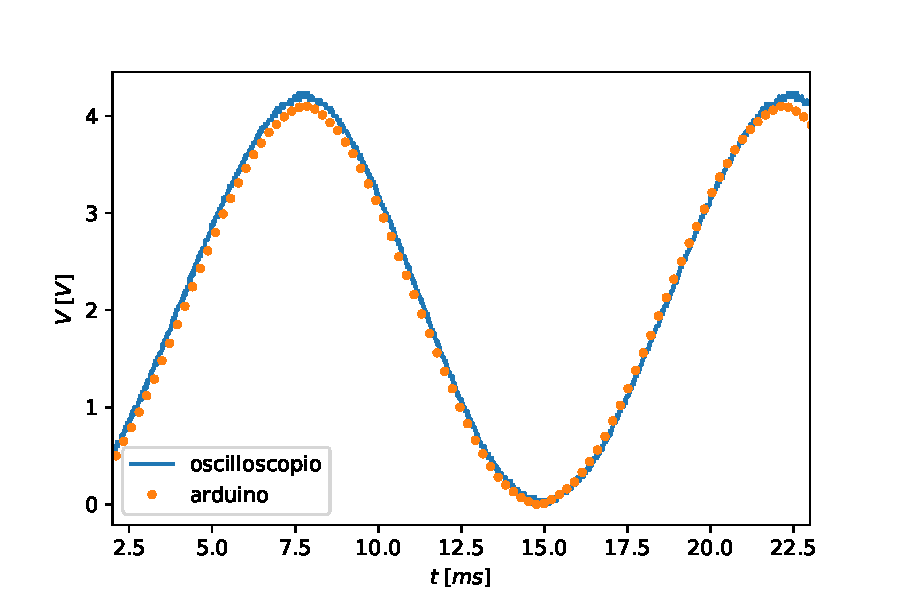
\includegraphics[width=\linewidth]{sinSovrapposta.pdf}
	\captionof{figure}{Onda sinusoidale misurata con Arduino sovrapposta alla misura di un oscilloscopio}
	\label{fig:ADC_sinusoidale}
	\end{center}
\end{Figure}

\begin{Figure}
	\begin{center}
	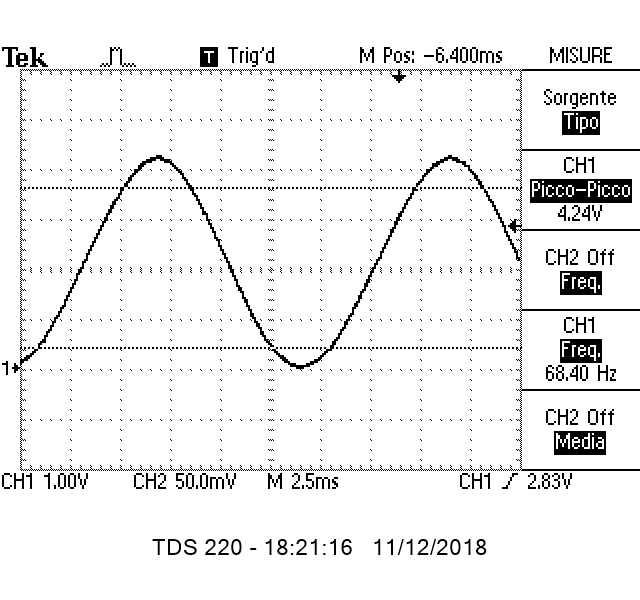
\includegraphics[width=\linewidth]{ingressoArduinoADCSin}
	\captionof{figure}{Istantanea dell'oscilloscopio per l'onda sinusoidale inviata all'Arduino}
	\label{fig:oscilloscopio_ADC_sinusoidale}
	\end{center}
\end{Figure}

Si ripete il campionamento per un segnale triangolare, di ampiezza picco-picco \SI{4.16 \pm 0.12}{V} e frequenza \SI{68 \pm 2}{\Hz}, e si riportano in Figura~\ref{fig:ADC_triangolare} il grafico di $V_x$ acquisita in funzione del tempo sovrapposto al segnale dell'oscilloscopio e in Figura~\ref{fig:oscilloscopio_ADC_triangolare} l'istantanea dell'oscilloscopio per questa configurazione.

\begin{Figure}
	\begin{center}
	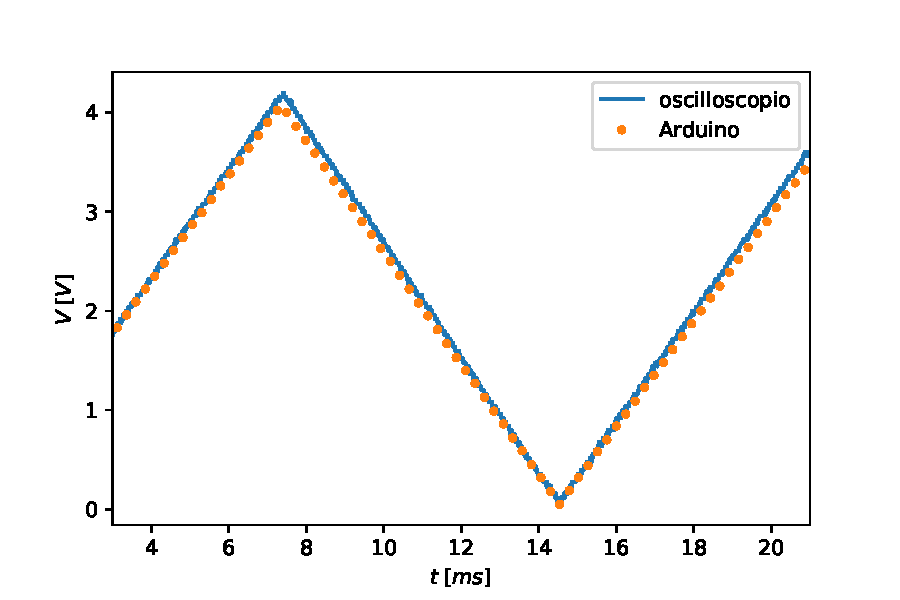
\includegraphics[width=\linewidth]{triangolareSovrapposta}
	\captionof{figure}{Onda triangolare misurata con Arduino sovrapposta alla misura di un oscilloscopio}
	\label{fig:ADC_triangolare}
	\end{center}
\end{Figure}

\begin{Figure}
	\begin{center}
	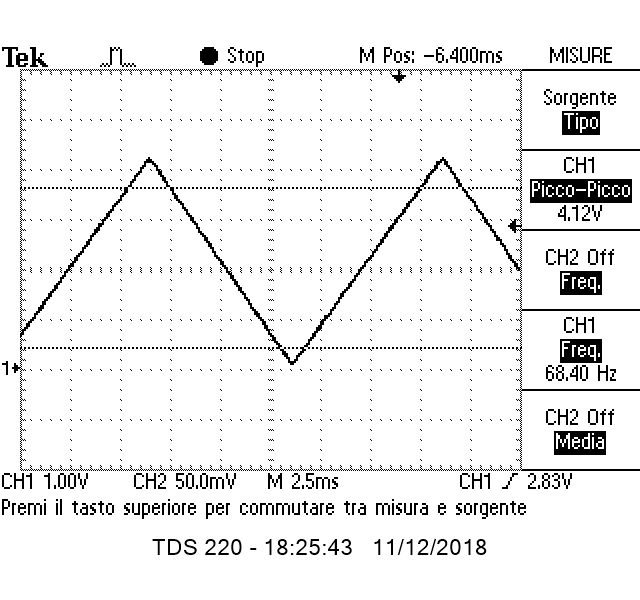
\includegraphics[width=\linewidth]{triangADC}
	\captionof{figure}{Istantanea dell'oscilloscopio per l'onda sinusoidale inviata all'Arduino}
	\label{fig:oscilloscopio_ADC_triangolare}
	\end{center}
\end{Figure}

Si osserva un buon accordo tra le misure fatte con la scheda Arduino e quelle fatte con l'oscilloscopio.




\end{multicols}
%\newpage
%\section{Appendice}


%ESEMPIO DI FIGURA
%\begin{Figure}
%	\begin{center}
%	\includegraphics[width=\linewidth]{comune.png}
%	\captionof{figure}{Istantanea dell'oscilloscopio per l'amplificatore differenziale, misura di $A_c$}
%	\label{fig:Ac_differenziale}
%	\end{center}
%\end{Figure}


%ESEMPIO DI TABELLA
%\begin{center}
%\captionof{table}{Misure per la stima di $A_c$}
%\label{tab:Ac_differenziale}
%\begin{tabular}{c|c|c|c}
%$f$ [\SI{}{Hz}] & $V_i$ [\SI{}{V}] & $v_o$ [\SI{}{mV}] & $A_c = v_o / V_i$ \\
%\hline
%      149.5 &        3.90 &         11.3 & 2.90e-03 \\
%      222.0 &        3.90 &         11.5 & 2.95e-03 \\
%      281.0 &        3.90 &         11.8 & 3.03e-03 \\
%      359.0 &        3.90 &         11.8 & 3.03e-03 \\
%      461.0 &        3.90 &         12.2 & 3.13e-03 \\
%\hline
%\end{tabular}
%\end{center}



\end{document}